% REMEMBER: You must not plagiarise anything in your report. Be extremely careful.

\documentclass{l4proj}
\usepackage {romannum}
\usepackage{tikz}
\usetikzlibrary{fit, matrix}

%
% put any additional packages here
%

\begin{document}

%==============================================================================
%% METADATA
\title{String Matching Algorithms Visualisation Software}
\author{Michal Wozniak}
\date{TO CHANGE}

\maketitle

%==============================================================================
%% ABSTRACT -  TO DO AT THE END
\begin{abstract}
    Every abstract follows a similar pattern. Motivate; set aims; describe work; explain results.
    \vskip 0.5em
    ``XYZ is bad. This project investigated ABC to determine if it was better.
    ABC used XXX and YYY to implement ZZZ. This is particularly interesting as XXX and YYY have
    never been used together. It was found that
    ABC was 20\% better than XYZ, though it caused rabies in half of subjects.''
\end{abstract}

%==============================================================================

% EDUCATION REUSE CONSENT FORM
% If you consent to your project being shown to future students for educational purposes
% then insert your name and the date below to  sign the education use form that appears in the front of the document.
% You must explicitly give consent if you wish to do so.
% If you sign, your project may be included in the Hall of Fame if it scores particularly highly.
%
% Please note that you are under no obligation to sign
% this declaration, but doing so would help future students.
%
\def\consentname {Michal Wozniak} % your full name
\def\consentdate {TO CHANGE} % the date you agree

\educationalconsent


%==============================================================================
\tableofcontents

%==============================================================================
%% Notes on formatting
%==============================================================================
% The first page, abstract and table of contents are numbered using Roman numerals and are not
% included in the page count.
%
% From now on pages are numbered
% using Arabic numerals. Therefore, immediately after the first call to \chapter we need the call
% \pagenumbering{arabic} and this should be called once only in the document.
%
% Do not alter the bibliography style.
%
% The first Chapter should then be on page 1. You are allowed 40 pages for a 40 credit project and 30 pages for a
% 20 credit report. This includes everything numbered in Arabic numerals (excluding front matter) up
% to but excluding the appendices and bibliography.
%
% You must not alter text size (it is currently 10pt) or alter margins or spacing.
%
%
%==================================================================================================================================
%
% IMPORTANT
% The chapter headings here are **suggestions**. You don't have to follow this model if
% it doesn't fit your project. Every project should have an introduction and conclusion,
% however.
%
%==================================================================================================================================
\chapter{Introduction}

% reset page numbering. Don't remove this!
\pagenumbering{arabic}


String search algorithms (otherwise known as string matching algorithms), such as Boyer-Moore (BM or BM Horsepool) and Knuth–Morris–Pratt (KMP) are pieces of code typically introduced at the higher education level for computer scientists, as well as students of related degrees. Quite simply, these aim to find the exact sequence of words or letters in longer pieces of text. Although commonly taught and used within various pieces of software, it can be hard to develop an intuition for their inner working. I, myself, have had a hard time getting to grips with how these work, having been taught these in my Algorithmics \Romannum{1} class during my third year of undergrad.

Many computer programs exist to facilitate a visual way to show the steps of such algorithms, however, I believe there is potential to create a product that not only reduces the learning complexity but also provides a novel, mobile-friendly application to help enthusiasts and students such as myself a few years ago to get a good understanding of the aforementioned and similar algorithms.

This document first aims to introduce the motivation behind the project,  explore existing software and determine the high-level aims and requirements for the project. What follows is the outline of the development process including the design and implementation steps as well as any decisions made for the benefit of the application or project management. The penultimate chapter explores how the prototype is perceived by the potential users at various stages of development to finally conclude how useful the final product is for the intended audience.


\section{Terminology}

Before discussing the project, it is important to highlight the terminology I will stick to throughout the document, as it can be quite loose between institutions and different documents online.  I will be using the term \textbf{pattern} to refer to the \textbf{sequence of words or characters we are searching for} and the word \textbf{text} to denote the \textbf{text we are searching within}.

\section{Motivation}

 % ubiquitous
 % anything with a computer
Sequences consisting of symbols and words are fundamental to society in the modern world according to Graham \citet{Stephen_1994}, an individual who dedicated a whole book to discussing string search algorithms. He states that grouping those to construct strings is one of the most natural concepts to a human. Not only are strings key in everyday communication, but in everything we do - think of what you are doing right now, making a shopping list, looking at the time, there is an infinite number of uses we encounter every day without even thinking about them.  String matching algorithms are a layer above strings, but ``judging by the wealth of published literature in this area \citep{Stephen_1994}'' these are just as foundational.

Although no longer the focus of today's development, they are vital for people within the technology field to understand in depth, as the knowledge simplifies construction and maintainance of software utilising them. The importance of the necessity to understand is further intensified by the number of modern tools utilising string matching algorithms in various fields, as denoted by \citet{GeeksforGeeks_2022}, such as:
\begin{itemize}
  \item \textbf{Plagiarism Detection} String matching algorithms are used to compare the content of 2 documents to establish similarity. Such tools are used throughout most stages of education to ensure work originality.
\item \textbf{Spelling Checkers} As with plagiarism detection, these can be particularly helpful in academia to ensure high-quality, spotless work.
  \item \textbf{DNA Sequencing} A lot of processes in the field of bioinformatics utilise string-matching facilities. One to highlight would be DNA pattern matching, which underpins gene analysis and helps determine potential illness, allowing for earlier and hence more effective treatment.
  \item \textbf{Digital Forensics} Official public bodies aim to prevent crimes against society, with string matching playing a vital role in supporting investigations by aiding information search on apprehended machines and law enforcement databases.
  \item \textbf{Spam Filters} Used by email services to help determine email importance by looking for specific words.
  \item \textbf{Search Engines} Used by most people everyday, matching algorithms underpin this procedure for query processing.
  \item \textbf{Intrusion Detection Systems In Software} In the cybersecurity field, we can analyse packets sent over a network by searching for malicious code based on known threats and malware.
\end{itemize}

\\


There is a plethora of established tools using string matching algorithms, however even now these search algorithms are used to drive innovation. A recent example would be the Intelligent Predictive String Search Algorithm created by \cite{GURUNG2016161}, which eliminates the need for pre-processing and works based on comparing the first and last letter of the pattern. Results show that it performs comparably to existing algorithms, at times better, while requiring less space and being simpler to understand. Another, more recent example would be the research conducted \cite{Ibrahim2023}, where the 2 newly developed algorithms had up to a 54\% performance increase compared to any other alternatives within the bio-informatics sphere.
\\


Most work today is based on the continued improvement of the performance of the information search process, due to the exponential increase of data available for analysis, as found by \cite{HASHEM201598} and his team while reviewing the rise of cloud computing . Henceforth understanding of the current algorithms is vital to being able to design new ones, but also to work with the vast amount of software using them. My application will aim to ease the process of learning the workflow undertaken by the principal string matching algorithms, to help gauge a deep understanding that can benefit individuals in the future.

\chapter{Background}
Before determining the requirements for creating my product, it is important to introduce the foundational string matching algorithms and explore existing visualisation solutions to establish the what my product should have.

\section{String Matching Algorithms}

As mentioned, string matching algorithms have the role of finding a specific set of symbols within a larger text. The are various algorithms developed over the years, all with their own advantages and drawbacks. I will be introducing the principal three algorithms, specifically the naive approach, Knuth-Morris-Pratt and Boyer-Moore.


\subsection{Brute Force Approach}
\label{alg:brute-force}
The naive approach involves going over each character in text and starting from such character, checking if each subsequent character matches the corresponding pattern character, if we assume the starting character corresponds to starting character of the pattern. This is done by incrementing the index of the text and pattern by 1 upon a match or upon a mismatch moving onto the next character of the text and resetting to the start of the pattern. If all symbols of the pattern match we can report a find, terminating the algorithm, otherwise we return something indicating failure in terms of the search. The pseudocode for this approach can be seen below, in Listing \ref{lst:brute}.

\lstinputlisting[label = {lst:brute}, caption=Brute Force Pseudocode, frame=single, columns=fullflexible]{code/brute-force.txt}

The time complexity of this algorithm is $O(mn)$, assuming n is the length of text and m is the length of the pattern. Such complexity arises from the fact that in the worst case (i.e. no match, but we will still need to compare the full length of pattern at each character of text , as the mismatch always occurs on the last character of pattern) we will need to go iterate over all characters in the text and all characters in the pattern at each iteration. The space complexity is constant ($O(1)$), as we only keep track of the $patternIndex$ and $textIndex$.
\\
\\
Such approach is trivial, however it can form a basis for introducing the problem of searching large pieces of text efficiently and highlight the need of more sophisticated methods such as ones introduced in the following sections.


\subsection{Knuth-Morris-Pratt}

Knuth-Morris-Pratt greatly improves upon its predecessor described in \ref{alg:brute-force} by achieving a linear time complexity of $O(m+n)$ in the worst case, paying for it with the increased space complexity of  $O(m)$ to store pre-processing results. Created by Donald Knuth, Vaughan Pratt, and by James H. Morris and published in 1977 (see \cite{KMP}), it is an online algorithm which exploits a border table in order to avoid backtracking within the text.
\\

\subsubsection{Pre-Processing}
The algorithm works on the basis of having the border table tell the system which pattern character should be compared with the current text character at the next step. The border table is a a data structure equal in length to the pattern, with each index representing a substring of the pattern up to, but excluding  character at that index. For example in the string of ababaca, the index of 4 assuming 0-indexing would consider the string of ababa, as denoted by the red outline in \ref{fig:kmp-pre-process} . Each entry of the structure contains the size of the substring that is both a prefix and suffix up to the relevant character of the pattern. Considering our earlier example of index 4 the prefix and suffix would be ab, which has a length of 2, as the first two characters are ab and the last two characters are also ab, denoted in blue and orange respectively.

\begin{figure}[hpt]
  \centering
  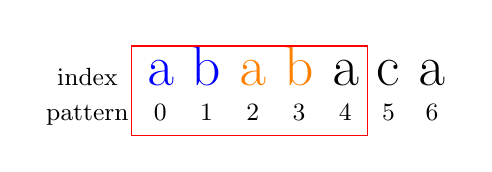
\begin{tikzpicture}
    [every node/.style={anchor=base, font=\huge},
     smallnum/.style={font=\small},
     textsize/.style={font=\small}]

    \matrix (m) [matrix of nodes, nodes in empty cells]
    {
      |[textsize]| index & |[text=blue]| a & |[text=blue]| b &  |[text=orange]| a & |[text=orange]| b & a & c & a \\
      |[textsize]| pattern & |[smallnum]| 0 & |[smallnum]| 1 & |[smallnum]| 2 & |[smallnum]| 3 & |[smallnum]| 4 & |[smallnum]| 5 & |[smallnum]| 6 \\
    };

    \node[fit=(m-1-2.north west) (m-2-6.south east), draw=red, inner sep=2pt] {};
  \end{tikzpicture}
  \caption{Working out border of pattern at index 4}
  \label{fig:kmp-pre-process}
\end{figure}

\subsubsection{Match}
Upon a match, as with the brute force algorithm we simply move one unit along within the text and the pattern.
\\

\subsubsection{Mismatch} There are 2 possible cases for KMP to consider when we fail to match 2 corresponding symbols. The case is determined on the basis of the border table. More specifically we index the border table using the current index of the pattern we mismatched on.  If the border table reports a result of a 0, we simply move one along in the text, since there is no prefix of the pattern that can match the already matched characters (the suffix). Such case is show visually in \ref{kmp:mismatch-case-1}.
Contrasting when the border table reports a non-zero value, it means the last $x$ characters in the already matched characters, match the start of the pattern. In such case we stay on the current character of the text, but shift the pattern to match the start of it with the aforementioned matching $x$ characters in the text. Visually this can be seen in \ref{kmp:mismatch-case-2}, where upon a mismatch of c and b, we work out the border of the pattern at c, which is 'aba'. We therefore need to move the pattern in a way where its start of aba, matches the already matched aba at the end of the text chunk we looked through so far.



\begin{figure}[hpt]
    \centering
    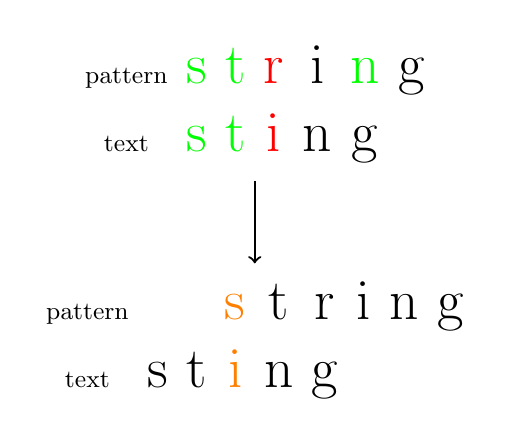
\begin{tikzpicture}
        [every node/.style={anchor=base, font=\huge},
        smallnum/.style={font=\small},
        textsize/.style={font=\small}]

    \begin{scope}
      \matrix (m) [matrix of nodes, nodes in empty cells]
      {
        |[textsize]| pattern & |[text=green]| s & |[text=green]| t &  |[text=red]| r &  i &
        |[text=green]| n &  g \\
      |[textsize]| text & |[text=green]| s & |[text=green]| t &  |[text=red]| i & n &  g \\
      };

    \end{scope}

     \begin{scope}[yshift=-3cm]
      \matrix (m1) [matrix of nodes, nodes in empty cells]
      {
        |[textsize]| pattern &
         &
         &
        |[text=orange]| s & t &  r &  i &
        n & g \\
      |[textsize]| text & s &  t &  |[text=orange]| i & n &
        g \\
      };
    \end{scope}

    \draw[->,thick] (m.south) -- (m1.north);
    \end{tikzpicture}
    \caption{KMP Mismatch - Case 1}
    \label{kmp:mismatch-case-1}
\end{figure}


\begin{figure}[hpt]
  \centering
  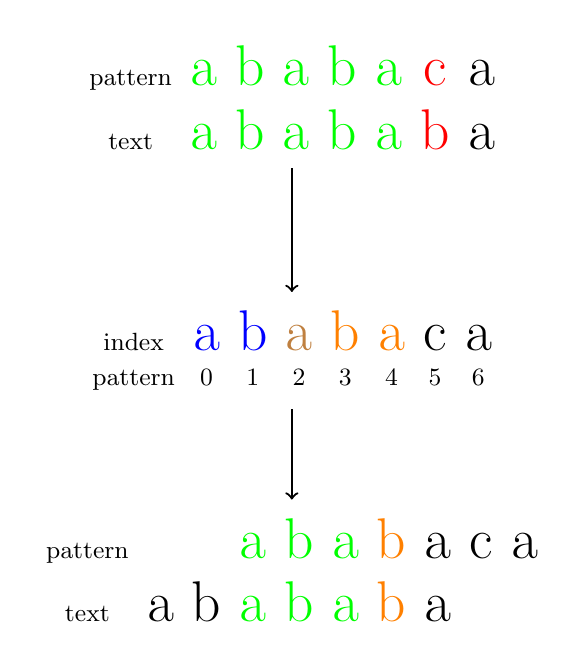
\begin{tikzpicture}
    [every node/.style={anchor=base, font=\huge},
     smallnum/.style={font=\small},
     textsize/.style={font=\small}]

    \begin{scope}
      \matrix (m1) [matrix of nodes, nodes in empty cells]
      {
        |[textsize]| pattern & |[text=green]| a & |[text=green]| b &  |[text=green]| a & |[text=green]| b &
        |[text=green]| a &
        |[text=red]|c & a \\
      |[textsize]| text & |[text=green]| a & |[text=green]| b &  |[text=green]| a & |[text=green]| b &
        |[text=green]| a &
        |[text=red]|b & a \\
      };

    \end{scope}

    \begin{scope} [yshift=-3cm]
    \matrix (m) [matrix of nodes, nodes in empty cells]
    {
      |[textsize]| index & |[text=blue]| a & |[text=blue]| b &  |[text=brown]| a & |[text=orange]| b & |[text=orange]| a & c & a \\
      |[textsize]| pattern & |[smallnum]| 0 & |[smallnum]| 1 & |[smallnum]| 2 & |[smallnum]| 3 & |[smallnum]| 4 & |[smallnum]| 5 & |[smallnum]| 6 \\
    };

    \draw[->,thick] (m1.south) -- (m.north);
    \end{scope}

    \begin{scope}[yshift=-6cm]
      \matrix (m2) [matrix of nodes, nodes in empty cells]
      {
        |[textsize]| pattern &
         &
         &
        |[text=green]| a & |[text=green]| b &  |[text=green]| a & |[text=orange]| b &
        a & c & a \\
      |[textsize]| text &  a &  b &  |[text=green]| a & |[text=green]| b &
        |[text=green]| a &
        |[text=orange]|b & a \\
      };
    \end{scope}

    \draw[->,thick] (m.south) -- (m2.north);

  \end{tikzpicture}
  \caption{KMP Mismatch Case 2}
  \label{kmp:mismatch-case-2}
\end{figure}

The algorithm pseudocode involving all the cases is outlined below:
\lstinputlisting[label = {lst:brute}, caption=Knuth-Morris-Pratt Pseudocode, frame=single, columns=fullflexible]{code/brute-force.txt}


\subsection{Boyer-Moore Algorithm}

Boyer-Moore is an algorithm introduced in 1975 \cite{}, before the dawn of KMP. On paper it appears slower than its ancestor, as its worst time complexity is $O(nm)$, however it has been found that its performance is almost always better in practice. The reason for such phenomenon is the fact BM is prone to skipping many characters per step, quickly eliminating areas of the text that cannot possibly match the pattern. Recently \cite{KMPvsBM} showed that BM outperformed KMP almost every single time , in some cases reaching one third of time it takes KMP to run.  Same as KMP , the algorithm is utilises a pre-processing data structure, which determines the next comparison during execution.
\\
\\
Unlike the 2 previous algorithms, it works on the basis of comparing right to left, starting the comparison from the last character in the pattern.

\subsubsection{Pre-Processing} During pre-processing a last occurrence table is create. Such data structure simply stores the last index of each character in the pattern.
\\

\subsubsection{Match} Upon a match, as with previous 2 algorithms introduced, there is one step forward in the text and the pattern.
\\

\subsubsection{Mismatch} Upon a mismatch, there are 3 possible things that can happen during execution.
\begin{itemize}
  \item \textbf{Case 1 - Last Occurrence of mismatched character has not been matched yet}
  When the last occurrence is to the left of the mismatched element of the pattern, we need to shift the pattern in such way to line up the last occurrence with the current text element we are looking at.  Referring to example in \ref{bm:mismatch-case-1}, we need the a in the pattern to be moved to the right until lined up with the mismatched a in the test.
  \item \textbf{Case 2 - Last Occurrence of the mismatched character has already been matched} In such case we simply move the pattern one place forward respective to the text (increment the $textIndex$ by 1)and restart the search from the end of the string. This happens because we cannot guarantee no match, since there could be another instance of the character within the pattern to match the text.
  \item \textbf{Case 3 - No last occurance, the character does not appear in the pattern} In such case we we move the pattern past the mismatched element i.e. we start checking the text from the next element, as it is impossible to match any substring where the pattern character does not exist.
\end{itemize}

The 3 cases combined make up the following pseudocode for the algorithm:
\lstinputlisting[label = {lst:brute}, caption=Boyer-Moore Pseudocode, frame=single, columns=fullflexible]{code/boyer-moore.txt}


\begin{figure}[hpt]
  \centering
  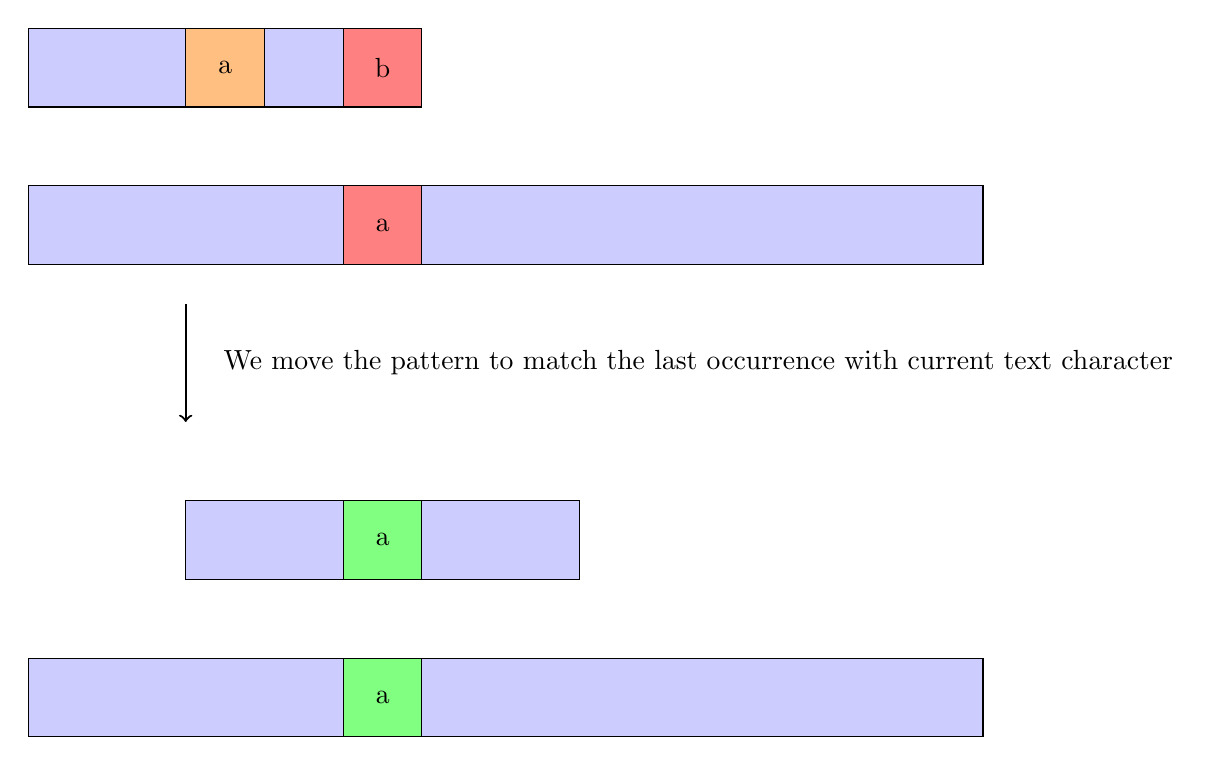
\begin{tikzpicture}
    \begin{scope}
        \draw [draw=black, fill=blue!20] (0,0) rectangle (4,1);
        \draw [draw=black, fill=red!50] (4, 0) rectangle (5, 1) node[midway] {b};;
        \draw [draw=black, fill=orange!50] (2,0) rectangle (3,1) node[midway] {a};
        \draw [draw=black, fill=blue!20] (0, -2) rectangle (\textwidth, -1);
        \draw [draw=black, fill=red!50] (4, -2) rectangle (5, -1) node[midway] {a};;
    \end{scope}

    \draw[->, thick] (2, -2.5) -- (2, -4)  node[midway, right, xshift=10pt] {We move the pattern to match the last occurrence with current text character};

    \begin{scope}
        \draw [draw=black, fill=blue!20] (2,-6) rectangle (7,-5);
        \draw [draw=black, fill=green!50] (4,-6) rectangle (5,-5) node[midway] {a};;
        \draw [draw=black, fill=blue!20] (0, -8) rectangle (\textwidth, -7);
        \draw [draw=black, fill=green!50] (4, -8) rectangle (5, -7) node[midway] {a};;
    \end{scope}
  \end{tikzpicture}
  \caption{Boyer-Moore Mismatch Case 1}
  \label{fig:boyer-moore-case-1}
\end{figure}



% \section{High Level Aims}

% The aim of the project is to develop a web application that will enable people to walk through the inner-working of string matching algorithms, with the aim of teaching. In line with the aim, the following high-level goals have been set:

% \begin{itemize}
%     \item \textbf{Naive Approach} Implement the naive approach visualisation to help people understand why such a method is not efficient
%     \item \textbf{Boyer-Moore} Implement the BM string search algorithm to highlight how pre-processing can be used to increase the efficiency of the search
%     \item \textbf{Knuth-Morris-Pratt} Implement the KMP algorithm to demonstrate how certain heuristics can be used to improve search efficiency.
%     \item \textbf{UI} Design a UI that will be easy to use, making it simple to start learning.
%     \item \textbf{Animations} The animations for all algorithms should be detailed, but also straightforward to understand.
%     \item \textbf{Software} The software should be well-tested, documented and well-designed making the process of implementing extra algorithms easygoing.
% 	\item \textbf{Evaluation} Throughout the development process I would like to conduct frequent evaluation sessions with potential users to ensure frequent feedback and hopefully improved satisfaction in my project so that it can end up being useful.

% \end{itemize}


% \section{Guidance}

% \textbf{Motivate} first, then state the general problem clearly.

% \section{Writing guidance}
% \subsection{Who is the reader?}

% This is the key question for any writing. Your reader:

% \begin{itemize}
%     \item
%     is a trained computer scientist: \emph{don't explain basics}.
%     \item
%     has limited time: \emph{keep on topic}.
%     \item
%     has no idea why anyone would want to do this: \emph{motivate clearly}
%     \item
%     might not know \emph{anything} about your project in particular:
%     \emph{explain your project}.
%     \item
%     but might know precise details and check them: \emph{be precise and
%     strive for accuracy.}
%     \item
%     doesn't know or care about you: \emph{personal discussions are
%     irrelevant}.
% \end{itemize}

% Remember, you will be marked by your supervisor and one or more members
% of staff. You might also have your project read by a prize-awarding
% committee or possibly a future employer. Bear that in mind.

% \subsection{References and style guides}
% There are many style guides on good English writing. You don't need to
% read these, but they will improve how you write.

% \begin{itemize}
%     \item
%     \emph{How to write a great research paper} \cite{Pey17} (\textbf{recommended}, even though you aren't writing a research paper)
%     \item
%     \emph{How to Write with Style} \cite{Von80}. Short and easy to read. Available online.
%     \item
%     \emph{Style: The Basics of Clarity and Grace} \cite{Wil09} A very popular modern English style guide.
%     \item
%     \emph{Politics and the English Language} \cite{Orw68}  A famous essay on effective, clear writing in English.
%     \item
%     \emph{The Elements of Style} \cite{StrWhi07} Outdated, and American, but a classic.
%     \item
%     \emph{The Sense of Style} \cite{Pin15} Excellent, though quite in-depth.
% \end{itemize}

% \subsubsection{Citation styles}

% \begin{itemize}
% \item If you are referring to a reference as a noun, then cite it as: ``\citet{Orw68} discusses the role of language in political thought.''
% \item If you are referring implicitly to references, use: ``There are many good books on writing \citep{Orw68, Wil09, Pin15}.''
% \end{itemize}

% There is a complete guide on good citation practice by Peter Coxhead available here: \url{http://www.cs.bham.ac.uk/~pxc/refs/index.html}.
% If you are unsure about how to cite online sources, please see this guide: \url{https://student.unsw.edu.au/how-do-i-cite-electronic-sources}.

% \subsection{Plagiarism warning}

% \begin{highlight_title}{WARNING}

%     If you include material from other sources without full and correct attribution, you are commiting plagiarism. The penalties for plagiarism are severe.
%     Quote any included text and cite it correctly. Cite all images, figures, etc. clearly in the caption of the figure.
% \end{highlight_title}


% %==================================================================================================================================
% \chapter{Background}
% What did other people do, and how is it relevant to what you want to do?
% \section{Guidance}
% \begin{itemize}
%     \item
%       Don't give a laundry list of references.
%     \item
%       Tie everything you say to your problem.
%     \item
%       Present an argument.
%     \item Think critically; weigh up the contribution of the background and put it in context.
%     \item
%       \textbf{Don't write a tutorial}; provide background and cite
%       references for further information.
% \end{itemize}

% %==================================================================================================================================
% \chapter{Analysis/Requirements}
% What is the problem that you want to solve, and how did you arrive at it?
% \section{Guidance}
% Make it clear how you derived the constrained form of your problem via a clear and logical process.

% %==================================================================================================================================
% \chapter{Design}
% How is this problem to be approached, without reference to specific implementation details?
% \section{Guidance}
% Design should cover the abstract design in such a way that someone else might be able to do what you did, but with a different language or library or tool.

% %==================================================================================================================================
% \chapter{Implementation}
% What did you do to implement this idea, and what technical achievements did you make?
% \section{Guidance}
% You can't talk about everything. Cover the high level first, then cover important, relevant or impressive details.



% \section{General points}

% These points apply to the whole dissertation, not just this chapter.



% \subsection{Figures}
% \emph{Always} refer to figures included, like Figure \ref{fig:relu}, in the body of the text. Include full, explanatory captions and make sure the figures look good on the page.
% You may include multiple figures in one float, as in Figure \ref{fig:synthetic}, using \texttt{subcaption}, which is enabled in the template.



% % Figures are important. Use them well.
% \begin{figure}
%     \centering
%     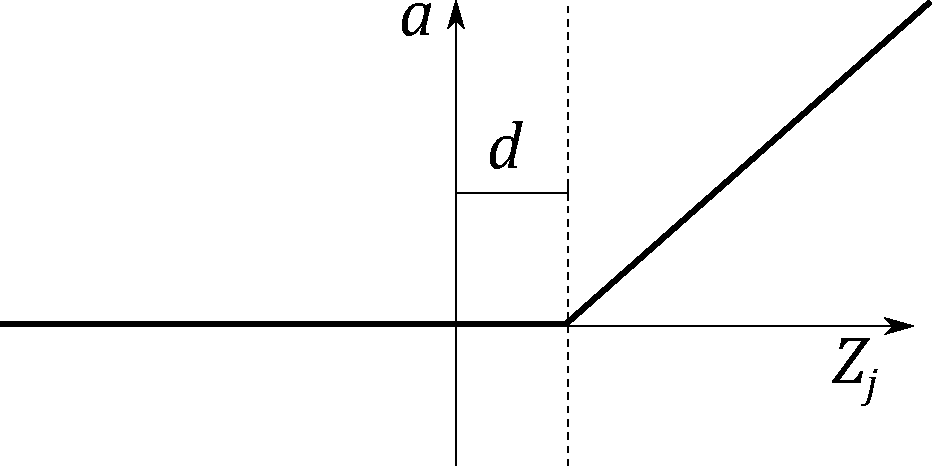
\includegraphics[width=0.5\linewidth]{images/relu.pdf}

%     \caption{In figure captions, explain what the reader is looking at: ``A schematic of the rectifying linear unit, where $a$ is the output amplitude,
%     $d$ is a configurable dead-zone, and $Z_j$ is the input signal'', as well as why the reader is looking at this:
%     ``It is notable that there is no activation \emph{at all} below 0, which explains our initial results.''
%     \textbf{Use vector image formats (.pdf) where possible}. Size figures appropriately, and do not make them over-large or too small to read.
%     }

%     % use the notation fig:name to cross reference a figure
%     \label{fig:relu}
% \end{figure}


% \begin{figure}
%     \centering
%     \begin{subfigure}[b]{0.45\textwidth}
%         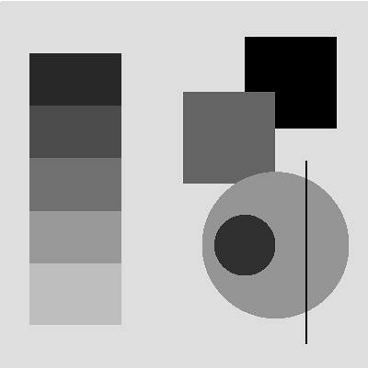
\includegraphics[width=\textwidth]{images/synthetic.png}
%         \caption{Synthetic image, black on white.}
%         \label{fig:syn1}
%     \end{subfigure}
%     ~ %add desired spacing between images, e. g. ~, \quad, \qquad, \hfill etc.
%       %(or a blank line to force the subfigure onto a new line)
%     \begin{subfigure}[b]{0.45\textwidth}
%         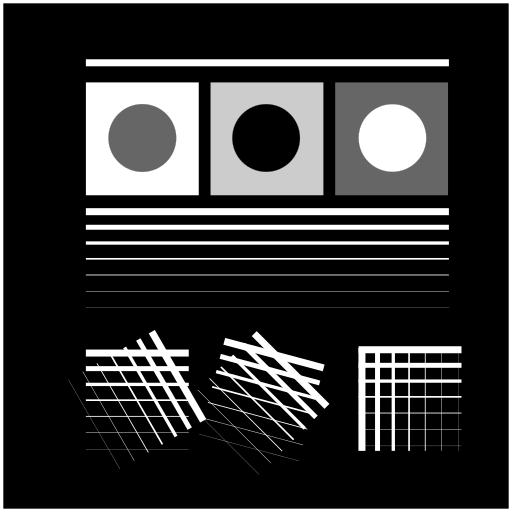
\includegraphics[width=\textwidth]{images/synthetic_2.png}
%         \caption{Synthetic image, white on black.}
%         \label{fig:syn2}
%     \end{subfigure}
%     ~ %add desired spacing between images, e. g. ~, \quad, \qquad, \hfill etc.
%     %(or a blank line to force the subfigure onto a new line)
%     \caption{Synthetic test images for edge detection algorithms. \subref{fig:syn1} shows various gray levels that require an adaptive algorithm. \subref{fig:syn2}
%     shows more challenging edge detection tests that have crossing lines. Fusing these into full segments typically requires algorithms like the Hough transform.
%     This is an example of using subfigures, with \texttt{subref}s in the caption.
%     }\label{fig:synthetic}
% \end{figure}

% \clearpage

% \subsection{Equations}

% Equations should be typeset correctly and precisely. Make sure you get parenthesis sizing correct, and punctuate equations correctly
% (the comma is important and goes \textit{inside} the equation block). Explain any symbols used clearly if not defined earlier.

% For example, we might define:
% \begin{equation}
%     \hat{f}(\xi) = \frac{1}{2}\left[ \int_{-\infty}^{\infty} f(x) e^{2\pi i x \xi} \right],
% \end{equation}
% where $\hat{f}(\xi)$ is the Fourier transform of the time domain signal $f(x)$.

% \subsection{Algorithms}
% Algorithms can be set using \texttt{algorithm2e}, as in Algorithm \ref{alg:metropolis}.

% % NOTE: line ends are denoted by \; in algorithm2e
% \begin{algorithm}
%     \DontPrintSemicolon
%     \KwData{$f_X(x)$, a probability density function returing the density at $x$.\; $\sigma$ a standard deviation specifying the spread of the proposal distribution.\;
%     $x_0$, an initial starting condition.}
%     \KwResult{$s=[x_1, x_2, \dots, x_n]$, $n$ samples approximately drawn from a distribution with PDF $f_X(x)$.}
%     \Begin{
%         $s \longleftarrow []$\;
%         $p \longleftarrow f_X(x)$\;
%         $i \longleftarrow 0$\;
%         \While{$i < n$}
%         {
%             $x^\prime \longleftarrow \mathcal{N}(x, \sigma^2)$\;
%             $p^\prime \longleftarrow f_X(x^\prime)$\;
%             $a \longleftarrow \frac{p^\prime}{p}$\;
%             $r \longleftarrow U(0,1)$\;
%             \If{$r<a$}
%             {
%                 $x \longleftarrow x^\prime$\;
%                 $p \longleftarrow f_X(x)$\;
%                 $i \longleftarrow i+1$\;
%                 append $x$ to $s$\;
%             }
%         }
%     }

% \caption{The Metropolis-Hastings MCMC algorithm for drawing samples from arbitrary probability distributions,
% specialised for normal proposal distributions $q(x^\prime|x) = \mathcal{N}(x, \sigma^2)$. The symmetry of the normal distribution means the acceptance rule takes the simplified form.}\label{alg:metropolis}
% \end{algorithm}

% \subsection{Tables}

% If you need to include tables, like Table \ref{tab:operators}, use a tool like https://www.tablesgenerator.com/ to generate the table as it is
% extremely tedious otherwise.

% \begin{table}[]
%     \caption{The standard table of operators in Python, along with their functional equivalents from the \texttt{operator} package. Note that table
%     captions go above the table, not below. Do not add additional rules/lines to tables. }\label{tab:operators}
%     %\tt
%     \rowcolors{2}{}{gray!3}
%     \begin{tabular}{@{}lll@{}}
%     %\toprule
%     \textbf{Operation}    & \textbf{Syntax}                & \textbf{Function}                            \\ %\midrule % optional rule for header
%     Addition              & \texttt{a + b}                          & \texttt{add(a, b)}                                    \\
%     Concatenation         & \texttt{seq1 + seq2}                    & \texttt{concat(seq1, seq2)}                           \\
%     Containment Test      & \texttt{obj in seq}                     & \texttt{contains(seq, obj)}                           \\
%     Division              & \texttt{a / b}                          & \texttt{div(a, b) }  \\
%     Division              & \texttt{a / b}                          & \texttt{truediv(a, b) } \\
%     Division              & \texttt{a // b}                         & \texttt{floordiv(a, b)}                               \\
%     Bitwise And           & \texttt{a \& b}                         & \texttt{and\_(a, b)}                                  \\
%     Bitwise Exclusive Or  & \texttt{a \textasciicircum b}           & \texttt{xor(a, b)}                                    \\
%     Bitwise Inversion     & \texttt{$\sim$a}                        & \texttt{invert(a)}                                    \\
%     Bitwise Or            & \texttt{a | b}                          & \texttt{or\_(a, b)}                                   \\
%     Exponentiation        & \texttt{a ** b}                         & \texttt{pow(a, b)}                                    \\
%     Identity              & \texttt{a is b}                         & \texttt{is\_(a, b)}                                   \\
%     Identity              & \texttt{a is not b}                     & \texttt{is\_not(a, b)}                                \\
%     Indexed Assignment    & \texttt{obj{[}k{]} = v}                 & \texttt{setitem(obj, k, v)}                           \\
%     Indexed Deletion      & \texttt{del obj{[}k{]}}                 & \texttt{delitem(obj, k)}                              \\
%     Indexing              & \texttt{obj{[}k{]}}                     & \texttt{getitem(obj, k)}                              \\
%     Left Shift            & \texttt{a \textless{}\textless b}       & \texttt{lshift(a, b)}                                 \\
%     Modulo                & \texttt{a \% b}                         & \texttt{mod(a, b)}                                    \\
%     Multiplication        & \texttt{a * b}                          & \texttt{mul(a, b)}                                    \\
%     Negation (Arithmetic) & \texttt{- a}                            & \texttt{neg(a)}                                       \\
%     Negation (Logical)    & \texttt{not a}                          & \texttt{not\_(a)}                                     \\
%     Positive              & \texttt{+ a}                            & \texttt{pos(a)}                                       \\
%     Right Shift           & \texttt{a \textgreater{}\textgreater b} & \texttt{rshift(a, b)}                                 \\
%     Sequence Repetition   & \texttt{seq * i}                        & \texttt{repeat(seq, i)}                               \\
%     Slice Assignment      & \texttt{seq{[}i:j{]} = values}          & \texttt{setitem(seq, slice(i, j), values)}            \\
%     Slice Deletion        & \texttt{del seq{[}i:j{]}}               & \texttt{delitem(seq, slice(i, j))}                    \\
%     Slicing               & \texttt{seq{[}i:j{]}}                   & \texttt{getitem(seq, slice(i, j))}                    \\
%     String Formatting     & \texttt{s \% obj}                       & \texttt{mod(s, obj)}                                  \\
%     Subtraction           & \texttt{a - b}                          & \texttt{sub(a, b)}                                    \\
%     Truth Test            & \texttt{obj}                            & \texttt{truth(obj)}                                   \\
%     Ordering              & \texttt{a \textless b}                  & \texttt{lt(a, b)}                                     \\
%     Ordering              & \texttt{a \textless{}= b}               & \texttt{le(a, b)}                                     \\
%     % \bottomrule
%     \end{tabular}
%     \end{table}
% \subsection{Code}

% Avoid putting large blocks of code in the report (more than a page in one block, for example). Use syntax highlighting if possible, as in Listing \ref{lst:callahan}.

% \begin{lstlisting}[language=python, float, caption={The algorithm for packing the $3\times 3$ outer-totalistic binary CA successor rule into a
%     $16\times 16\times 16\times 16$ 4 bit lookup table, running an equivalent, notionally 16-state $2\times 2$ CA.}, label=lst:callahan]
%     def create_callahan_table(rule="b3s23"):
%         """Generate the lookup table for the cells."""
%         s_table = np.zeros((16, 16, 16, 16), dtype=np.uint8)
%         birth, survive = parse_rule(rule)

%         # generate all 16 bit strings
%         for iv in range(65536):
%             bv = [(iv >> z) & 1 for z in range(16)]
%             a, b, c, d, e, f, g, h, i, j, k, l, m, n, o, p = bv

%             # compute next state of the inner 2x2
%             nw = apply_rule(f, a, b, c, e, g, i, j, k)
%             ne = apply_rule(g, b, c, d, f, h, j, k, l)
%             sw = apply_rule(j, e, f, g, i, k, m, n, o)
%             se = apply_rule(k, f, g, h, j, l, n, o, p)

%             # compute the index of this 4x4
%             nw_code = a | (b << 1) | (e << 2) | (f << 3)
%             ne_code = c | (d << 1) | (g << 2) | (h << 3)
%             sw_code = i | (j << 1) | (m << 2) | (n << 3)
%             se_code = k | (l << 1) | (o << 2) | (p << 3)

%             # compute the state for the 2x2
%             next_code = nw | (ne << 1) | (sw << 2) | (se << 3)

%             # get the 4x4 index, and write into the table
%             s_table[nw_code, ne_code, sw_code, se_code] = next_code

%         return s_table

% \end{lstlisting}

% %==================================================================================================================================
% \chapter{Evaluation}
% How good is your solution? How well did you solve the general problem, and what evidence do you have to support that?

% \section{Guidance}
% \begin{itemize}
%     \item
%         Ask specific questions that address the general problem.
%     \item
%         Answer them with precise evidence (graphs, numbers, statistical
%         analysis, qualitative analysis).
%     \item
%         Be fair and be scientific.
%     \item
%         The key thing is to show that you know how to evaluate your work, not
%         that your work is the most amazing product ever.
% \end{itemize}

% \section{Evidence}
% Make sure you present your evidence well. Use appropriate visualisations, reporting techniques and statistical analysis, as appropriate.

% If you visualise, follow the basic rules, as illustrated in Figure \ref{fig:boxplot}:
% \begin{itemize}
% \item Label everything correctly (axis, title, units).
% \item Caption thoroughly.
% \item Reference in text.
% \item \textbf{Include appropriate display of uncertainty (e.g. error bars, Box plot)}
% \item Minimize clutter.
% \end{itemize}

% See the file \texttt{guide\_to\_visualising.pdf} for further information and guidance.

% \begin{figure}
%     \centering
%     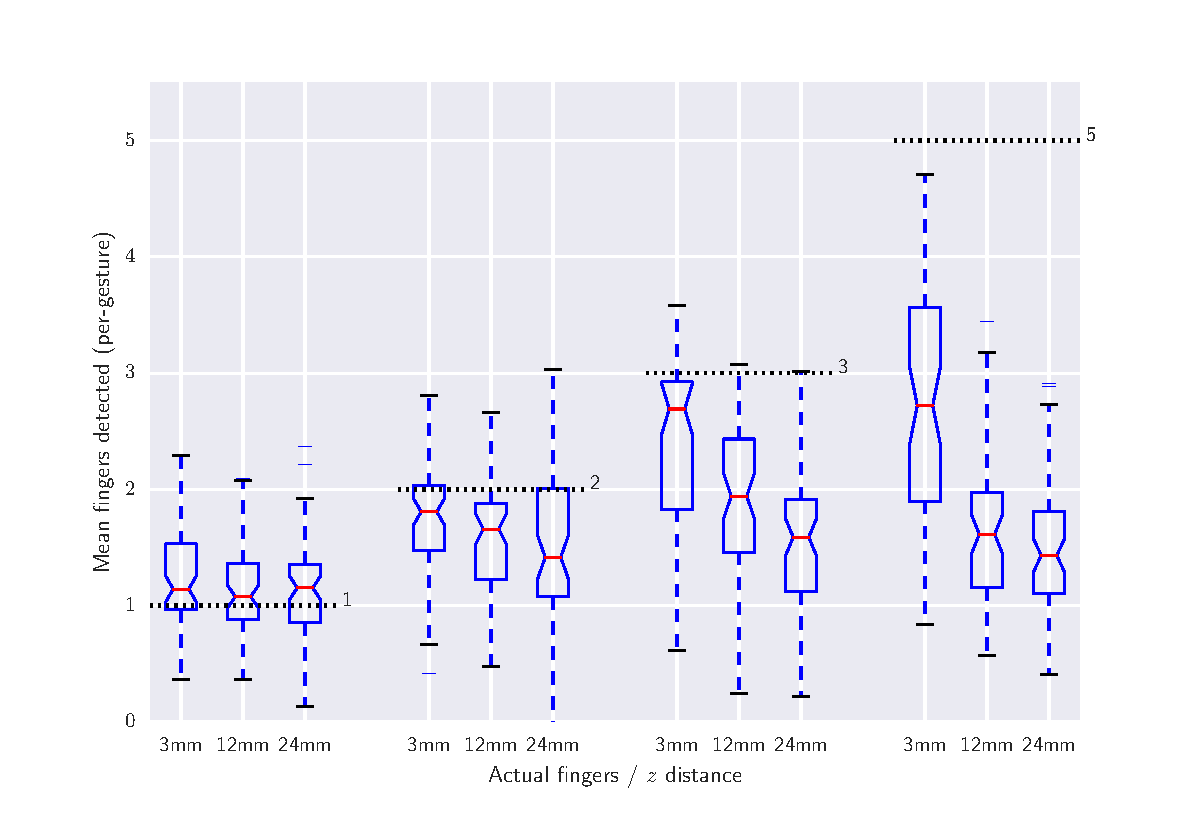
\includegraphics[width=1.0\linewidth]{images/boxplot_finger_distance.pdf}

%     \caption{Average number of fingers detected by the touch sensor at different heights above the surface, averaged over all gestures. Dashed lines indicate
%     the true number of fingers present. The Box plots include bootstrapped uncertainty notches for the median. It is clear that the device is biased toward
%     undercounting fingers, particularly at higher $z$ distances.
%     }

%     % use the notation fig:name to cross reference a figure
%     \label{fig:boxplot}
% \end{figure}


% %==================================================================================================================================
% \chapter{Conclusion}
% Summarise the whole project for a lazy reader who didn't read the rest (e.g. a prize-awarding committee).
% \section{Guidance}
% \begin{itemize}
%     \item
%         Summarise briefly and fairly.
%     \item
%         You should be addressing the general problem you introduced in the
%         Introduction.
%     \item
%         Include summary of concrete results (``the new compiler ran 2x
%         faster'')
%     \item
%         Indicate what future work could be done, but remember: \textbf{you
%         won't get credit for things you haven't done}.
% \end{itemize}

% %==================================================================================================================================
% %
% %
% %==================================================================================================================================
% %  APPENDICES

% \begin{appendices}

% \chapter{Appendices}

% Typical inclusions in the appendices are:

% \begin{itemize}
% \item
%   Copies of ethics approvals (required if obtained)
% \item
%   Copies of questionnaires etc. used to gather data from subjects.
% \item
%   Extensive tables or figures that are too bulky to fit in the main body of
%   the report, particularly ones that are repetitive and summarised in the body.

% \item Outline of the source code (e.g. directory structure), or other architecture documentation like class diagrams.

% \item User manuals, and any guides to starting/running the software.

% \end{itemize}

% \textbf{Don't include your source code in the appendices}. It will be
% submitted separately.

% \end{appendices}

%==================================================================================================================================
%   BIBLIOGRAPHY

% The bibliography style is abbrvnat
% The bibliography always appears last, after the appendices.

\bibliographystyle{abbrvnat}

\bibliography{l4proj}

\end{document}
